\chapter{Brudgrænsetilstand}
INDLEDNING

\section{Reaktioner}
Når der beregnes reaktionskræfter for de tre understøtninger, er der behov for at opdele konstruktionen. Systemet opdeles i det midterste charnierled i henholdvis en venstre- og højre del, som ses på Figur \ref{fig:opdelingv} og \ref{fig:opdelingh}. I skæringen mellem de to dele, vil der være snitkræfter men ikke momentkræfter, da momentet i charnierledet er nul. Dermed optræder der kun normalkraften, N, og forskydningskraften, V.

\begin{figure}[htbp]\centering
	\begin{minipage}[b]{0.48\textwidth}\centering
		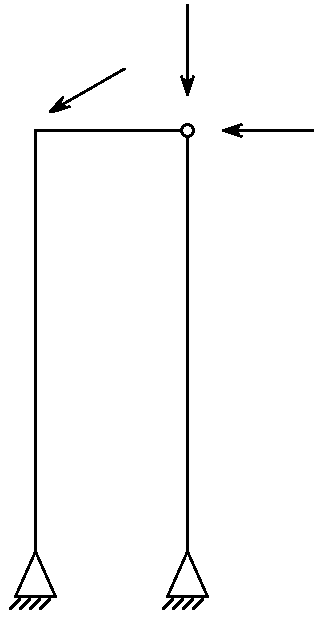
\includegraphics[width=0.50\textwidth]{billeder/venstre.png} %Venstre billede
	\end{minipage}\hfill
	\begin{minipage}[b]{0.48\textwidth}\centering
		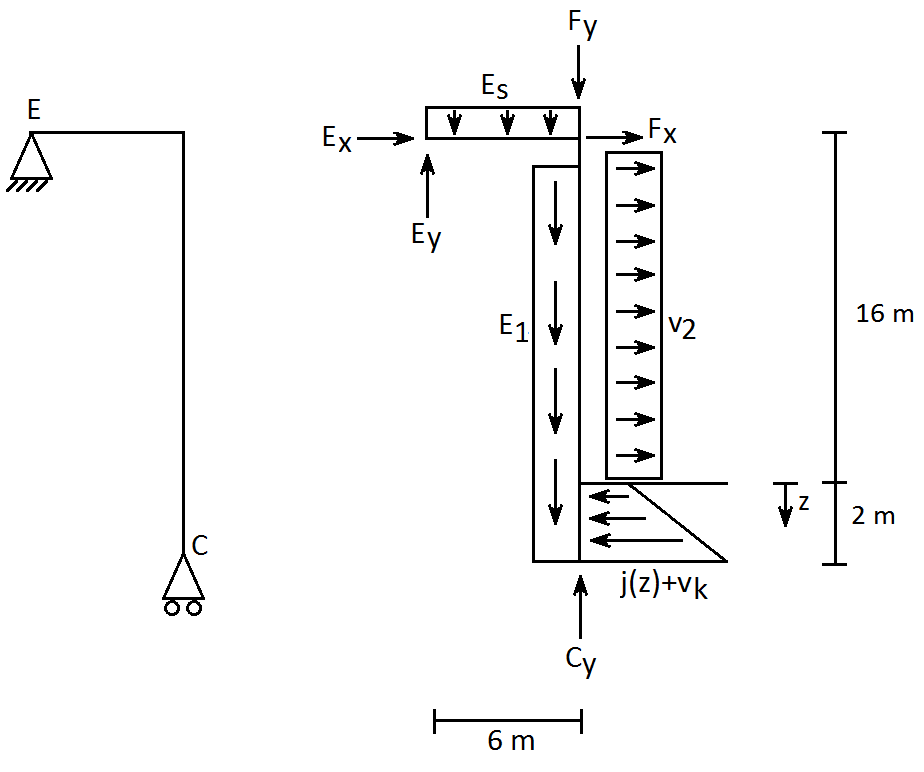
\includegraphics[width=0.35\textwidth]{billeder/hojre.png} %Højre billede
	\end{minipage}\\ %Captions and labels
	\begin{minipage}[t]{0.48\textwidth}
		\caption{Venstre side af systemet} %Venstre caption og label
		\label{fig:opdelingv}
	\end{minipage}\hfill
	\begin{minipage}[t]{0.48\textwidth}
		\caption{Højre side af systemet} %Højre caption og label
		\label{fig:opdelingh}
	\end{minipage}
\end{figure}

Reaktionerne, der vil virke i charnieret, sættes som belastninger på venstre del af systemet. 
\newline
\newline
Reaktionerne på højre del af systemet beregnes først.
\newline
\newline
Lasterne, der påvirker højre side af det statiske system, ses på Figur XX, hvor værdierne kan ses i Tabel \ref{tab:laster}.
% Indsæt figur med hvordan lasterne er på venstre- og højre del af systemet.

\begin{table}
	\begin{center}
		\begin{tabular}{|c|c|c|}
			\hline
Betegnelse     & Værdi & Enhed \\ \hline
$P_1$           &       &       \\ \hline
$P_2$           &       &       \\ \hline
$q_1$           & 31,54 & $\frac{kN}{m}$ \\ \hline
$q_2$           & 9,47  & $\frac{kN}{m}$ \\ \hline
$q_3$           & 61,34 & $\frac{kN}{m}$ \\ \hline
$Vind_1$        & 6,08  & $\frac{kN}{m}$ \\ \hline
$Vind_2$       	& -1,20 & $\frac{kN}{m}$ \\ \hline
$Jord+vind_ind$ & $63,\!77x + 1,\!66$ & $\frac{kN}{m}$ \\ \hline
		\end{tabular}
		\caption{Laster på det statiske system}
		\label{tab:laster}
	\end{center}
\end{table}

Først bestemmes den vandrette reaktion i charnier ledet, $S_v$ gennem vandret ligevægt: 
\begin{center}
	$\rightarrow+:0 = F_x + S_v - J(2m) - V_k \cdot 2m - V_2 \cdot 16m$
	$S_v \leftrightarrow -1309,\!49 N$
\end{center}

Nu bestemmes $C_y$ gennem moment ligevægt om punkt E: 
\begin{center}
	$\AR{}:0 = -F_y \cdot 6m - E_1 \cdot 18m \cdot 6m + C_y \cdot 6m - J(2m) \cdot 17,\!33m - V_k \cdot 2m \cdot 17m - E_s \cdot 6m \cdot 3m - V_2 \cdot 16m \cdot 8m$
\end{center}
\begin{center}
	$C_y = 7,\!80 \cdot 10^5 N$
\end{center}

Nu kan den lodrette reaktion i charnier ledet, $S_l$ bestemmes gennem lodret ligevægt: 
\begin{center}
	$\uparrow+: 0 = F_y - E_1 \cdot 18m - E_s \cdot 6m + C_y + S_l$
\end{center}
\begin{center}	
	$S_l = -2,\!44 \cdot 10^5N$
\end{center}

Nu er reaktionerne for det højre system bestemt, og disse sættes nu på som belastninger i punkt E for det venstre system, og reaktionerne bestemmes for dette. Da reaktionerne i begge systemer peger i negativ rentning, så ændres fortegnet og dermed retning, så de virker som vist på figur 4. ???

%indsæt Figur 

Først tages der moment om A, for at beregne $B_y$  
\begin{center}
	$A\hookrightarrow+: 0 = B_y \cdot 6m + S_l \cdot 6m + S_v \cdot 18m - E_2 \cdot 18m \cdot 6m - E_s \cdot 6m \cdot 3m + D_x \cdot 18m - V_1 \cdot 16m \cdot (8m + 2m) - J(2m) \cdot (2m \cdot \frac{1}{3}) - V_k \cdot 2m \cdot 1m$ 
	$B_y \leftrightarrow 9,\!49 \cdot 10^5N$
\end{center}

Nu laves lodret ligevægt for at bestemme $A_y$
\begin{center}
	$\uparrow+: 0 = A_y + B_y - S_l - E_2 \cdot 18m - E_1 \cdot 18m - F_y - E_s \cdot 6 m$
	$A_y \leftrightarrow 5,\!35 \cdot 10^5N$
\end{center}

For at gøre det muligt at isolere en af de vandrette reaktioner laves der et snint i charnieret, og derefter tages der moment omkring charnieret i punkt E, for at bestemme $B_x$.
\begin{center}
	$\hookrightarrow+: 0 = B_x \cdot 18m$
	$B_x \leftrightarrow 0N$
\end{center}

Slutteligt laves vandret ligevægt for at bestemme $A_x$
\begin{center}
	$\rightarrow+: 0 = A_x - S_v + B_x + J(2m) + V_k \cdot 2m + V_1 \cdot 16 m - D_x$
	$A_x \leftrightarrow -1,\!33 \cdot 10^5N$
\end{center} 
 
 Nu er reaktionerne bestemt for det statiske system, og der skal nu laves snitkræfter for system, både ved beregning af brudgrænsetilstanden og anvendelsesgrænsetilstanden. 
 
 
\section{Snitkræfter}
Både snitkræfter og snitkræftskurver.

\section{Spænding}
For at finde ud af om konstruktionen kan holde, undersøges spændingstilstanden. Her skal det gælde:

\begin{center}
	$\sqrt{\sigma^2 + 3\tau^2} \leq f_y$ 
\end{center}

\begin{itemize}
	\item[-] $\sigma$: Normalspænding
	\item[-] $\tau$: Forskydningsspænding
	\item[-] $f_y$: Flydespænding
\end{itemize}

Flydespændingen beregnes ved formlen:

\begin{center}
	$f_y = \frac{f_{yk}}{\gamma}$
\end{center}

\begin{itemize}
	\item[-] $f_{yk}$: Den karakteristiske flydespænding, der afhænger af ståltype. For ståltype S235 er $f_{yk} = 225 MPa$
	\item[-] $\gamma$: Partialkoefficient, der sættes til 1,1 \citep[ s. 212]{stabi}.  
\end{itemize}

Altså beregnes den regningsmæssige flydespænding til:

\begin{center}
	$f_y = \frac{225 MPa}{1,\!1} = 204,\!54 MPa$
\end{center}

Normalspændingen findes ved Naviers formel:

\begin{center}
	$\sigma = \frac{N}{A} - \frac{M}{I} y$
\end{center}

\begin{itemize}
	\item[-] N: Normalkraft [kN]
	\item[-] A: Tværsnitsareal, som for stålprofil 450 er $14,\!7 \cdot 10^3 mm^2$ \citep{stabi}. 
	\item[-] M: Moment [kN]
	\item[-] y: Tyngdepunktskoordinat [mm]
	\item[-] I: Inertimoment, som for stålprofil 450 er $458,\!5 \cdot 10^6 mm^4$ \citep{stabi}. 
\end{itemize} 

Dernæst beregnes forskydningsspændingen ved Grasshofs formel:

\begin{center}
	$\tau = \frac{VQ}{Ib}$
\end{center}

\begin{itemize}
	\item[-] V: Forskydningskraft [kN]
	\item[-] Q: 1. ordens arealmoment for $A_1$: $Q = \int_{A_1}y, \mathrm{d}A = yA$ $[mm^3]$
	\item[-] b: bredde
\end{itemize}

Nedenfor vises et beregningseksempel for et kritisk punkt. Resultaterne for alle de valgte kritiske punkter kan ses i tabel XX. 
\newline
\newline
VIS BEREGNINGSEKSEMPEL FOR ET KRITISK PUNKT
\newline
\newline
INDSÆT TABEL MED RESULTATER (SE MAPLE-DOKUMENT) 
\newline
\newline
SKRIV KONKLUSION (KAN DET HOLDE)? Hvad kan man gøre hvis det ikke kan holde - eller er det "overdimensioneret"?